% Author: David Larsen <dcl9934@cs.rit.edu>
% Author: Doug Krofcheck <dpk3062@rit.edu>
\documentclass[11pt]{article}
\usepackage{fullpage}
\usepackage{listings}
\usepackage{needspace}
\usepackage{color}
\usepackage{ifthen}
\usepackage{graphicx}
\usepackage{csc}
\usepackage{tikz}
\usetikzlibrary{shapes}

\lstset{ %
basicstyle=\footnotesize,       % the size of the fonts that are used for the code
numbers=left,                   % where to put the line-numbers
stepnumber=1,                   % the step between two line-numbers. If it's 1 each line will be numbered
numbersep=5pt,                  % how far the line-numbers are from the code
showspaces=false,               % show spaces adding particular underscores
showstringspaces=false,         % underline spaces within strings
tabsize=4,		                % sets default tabsize to 4 spaces
language=Python
}

\ifthenelse{\isundefined{\isAnswerKey}}
{
    \newenvironment{answer}{\large\lstset{basicstyle=\large}\color{white} \small{Answer:}\large}{}
}
{
    \newenvironment{answer}{\large\lstset{basicstyle=\large}\color{red} \small{Answer:}\large}{}
}

\title{CSCI-142 Midterm Exam Review}
\author{Computer Science Community}
\date{\today}

\makeatletter
\let\thetitle\@title
\let\theauthor\@author
\let\thedate\@date
\makeatother

\begin{document}
\header
\begin{enumerate}


\item What are you called by your peers? \\
\begin{answer}
(Student's callsigns/names may vary per student)
\end{answer}



\item Why can we not use {\tt ==} to determine if two strings are equivalent? \\
\begin{answer}
{\tt ==} will check to see if two objects are the exact same object. If we want to compare objects by meaning, they'll have to implement the {\tt Comparable} interface, which declares the {\tt equals} method. For strings we could say {\tt ``yes''.equals(``yes'')}.
\end{answer}



\item If an instance variable is declared with {\tt protected} access, who can access it? \\
\begin{answer}
Methods in that class and methods in all of its subclasses.
\end{answer}



\item What is the difference between a class and an object? \\
\begin{answer}
A class is a construct that defines methods and properties - it can be viewed as a template. An objects are instances of that class. Think of classes as molds and objects as individual things created by those molds.
\end{answer}



\item What is the difference between a constant and a normal variable? Give an example of a constant declaration. \\
\begin{answer}
A constant may never change during run time (it may be set {\em once}).
	\begin{lstlisting}
public static final int NUM_PEOPLE_WHO_LIKE_JAVA = 0;
	\end{lstlisting}
\end{answer}



\item What is the difference between overriding and overloading methods?  Give a example situation where each should be used. \\
\begin{answer}
Overriding: method with the exact same method declaration as a method in a superclass; overwrites and/or extends the functionality of the super() method
Overloading: 2 or more methods with the same name and return type that either:
	\begin{enumerate}
	\item have a different number of parameters\\ \textbf{OR}
	\item have parameters of different types
	\end{enumerate}
Override a method when you want to REPLACE the implementation of a method in a superclass.  Overload a method (such as a constructor) when you want to have more than one implementation of a method for different circumstances.
\end{answer}



\item Define polymorphism and explain a situation in which you would use it. \\
\begin{answer}
Polymorphism: the ability to create an object of more than one type. References and collections of a super class may hold instances of subclasses. Methods invoked on these objects determine the correct (type specific) behavior at runtime. \\
EX:
		\begin{lstlisting}
ArrayList<Shape> shapes = new ArrayList<Shape>();
shapes[0] = new Square(1);
shapes[1] = new Circle(9);
shapes[2] = new Triangle(4);
for( int i = 0; i < shapes.size(); i++ ){ 
   	double area = shapes[i].getArea();
   	System.out.println("" + area);
}
        \end{lstlisting}
\end{answer}



\item What is the difference between an abstract class and an interface? Why might you want to use an interface over an abstract class? \\
\begin{answer}
Abstract classes allow for default method behavior to be defined, while interfaces allow only method declaration.  Since java allows a class to extend only a single class but implement many interfaces, interfaces provide some extended capabilities. However, extending an abstract class allows usage of the defined default behaviors. 
\end{answer}


\newpage


\item What gets printed by the following code?
\begin{lstlisting}
public class Class1 {
	public Class1() {
		System.out.println( "Class1()" );
	}
	public void print1() {
		System.out.println( "Class1.print1()" );
	}
	public void print2() {
		System.out.println("Class1.print2()" );
	}
}

public class Class2 extends Class1 {
	public Class2() {
		System.out.println( "Class2()" );
	}
	public void print1() {
		System.out.println("Class2.print1()");
	}
}

public class Class3 extends Class1{
	private Class2 class2;
	public Class3() {
		System.out.println( "Class3()" );
		class2 = new Class2();
	}
	public void print1() {
		class2.print1();
	}
	public void print2(){
		System.out.println("Class3.print2()");
		super.print2();
	}
}

public class TestClass {
	public static void main( String[] args ) {
		Class1 c1 = new Class2();
		c1.print1();
		c1.print2();

		System.out.println();
		Class1 c2 = new Class3();
		c2.print1();
		c2.print2();
	}
}
\end{lstlisting}
\begin{answer}
    \begin{verbatim}
Class1()
Class2()
Class2.print1()
Class1.print2()

Class1()
Class3()
Class1()
Class2()
Class2.print1()
Class3.print2()
Class1.print2()
    \end{verbatim}
\end{answer}


\newpage


\item Find at least 3 errors related to inheritance and interfaces in the following code:\label{demolition-derby}
\begin{lstlisting}
public interface Vehicle {
	public int getSpeed();
	public void accelerate(int speed_increase);
	public void brake(int speed_decrease);
}
public class Car implements Vehicle {
	private int speed;
	public Car(int initialSpeed){
		this.speed = initialSpeed;
	}
	public int getSpeed(){
		return speed;
	}
	public int accelerate(int speed_increase) {
		speed += speed_increase;
	}
	public int brake(int speed_decrease) {
		speed -= speed_decrease;
	}
}
public class Toyota extends Car {
	public long getSpeed(){
		return speed;
	}
	public void brake(Integer speed_decrease) {}
	public void factoryRecall(){
		System.out.println("Replace my floor mat!");
	}
}
public class Truck implements Vehicle {
	public void accelerate(int speed_increase) {
		super.accelerate(speed_increase/2);
	}
	public void brake(int speed_decrease) {
		super.brake(speed_decrease/2);
	}
}
public class demolitonDerby {
	public static void main(String[] args) {
		Vechicle	prius, mack, impreza;
		prius = new Toyota();
		mack = new Truck();
		impreza = new Car();
		
		impreza.accelerate(5);
		prius.brake(2);
		prius.factoryRecall();
		prius.accelerate(impreza.getSpeed());
		mack.accelerate(5.0);
	}
\end{lstlisting}
\begin{answer}
    \begin{tabular}{r l} % TODO Fix some answers here
    Line \# & Error \\\hline
    14  	& Returns int, should return void\\
    17  	& Returns int, should return void\\
    22  	& getSpeed()'s return type ({\tt long}) differs from Car or Vehicle.\\
    23  	& speed is private.\\
    25,46	& Calling brake() on Toyotas will call the superclass's brake()\\
    30  	& Truck implements vehicle, but does not have getSpeed()\\
    32  	& Can't call super(), this has no superclass.\\
    33  	& Can't call super(), this has no superclass.\\
    47  	& {\tt prius} was declared as a {\tt Vehicle}, so we can't call\\
    ~  		& methods that aren't declared in {\tt Vehicle}.\\
    49  	& FIXME I don't think it's legal to pass a double to an int without casting.
    \end{tabular}
\end{answer}


\section*{Sorting}


\item Fill in the table for the asymptotic running time of each sorting algorithm.
\begin{center}
	\begin{tabular}{|r|c|c|c|} \hline
	~ & Best & Worst & Average \\\hline
	MergeSort &
		\begin{answer}$O(n*\textrm{log}(n))$\end{answer} &
		\begin{answer}$O(n*\textrm{log}(n))$\end{answer} &
		\begin{answer}$O(n*\textrm{log}(n))$\end{answer} \\\hline
	Quicksort &
		\begin{answer}$O(n*\textrm{log}(n))$\end{answer} &
		\begin{answer}$O(n^2)$\end{answer} &
		\begin{answer}$O(n*\textrm{log}(n))$\end{answer} \\\hline
	HeapSort &
		\begin{answer}$O(n*\textrm{log}(n))$\end{answer} &
		\begin{answer}$O(n*\textrm{log}(n))$\end{answer} &
		\begin{answer}$O(n*\textrm{log}(n))$\end{answer} \\\hline
	\end{tabular}
\end{center}



\item What sorting algorithm splits its input list into two other lists, one which has element which are all smaller than a value (which is randomly selected) and one which has elements which are all larger than the randomly selected value? \\
\begin{answer}
Quicksort.
\end{answer}



\item What kind of data causes Quicksort's worst-case time complexity? You may assume that we always pick the first element as the pivot. \\
\label{qsort-worst-case}
\begin{answer}
Data that is (nearly) sorted or is sorted in reverse order.
\end{answer}

\item What causes Quicksort to run so slowly on the input you describe in question \ref{qsort-worst case}? \\
\begin{answer}
Quicksort splits its input into two lists based on the value of the pivot.  If the pivot is either the smallest or the largest element, then one list will only have no elements, while the others will have all of the elements but the pivot. We can see this if we perform a substitution trace:
	\begin{verbatim}
	qsort([1,2,3,4])
	qsort([]) + [1] + qsort([2,3,4])
	qsort([]) + [1] + qsort([]) + [2] + qsort([3,4])
	qsort([]) + [1] + qsort([]) + [2] + qsort([]) + [3] + qsort([4])
	qsort([]) + [1] + qsort([]) + [2] + qsort([]) + [3] + qsort([4])
	qsort([]) + [1] + qsort([]) + [2] + qsort([]) + [3] + qsort([]) + [4] + qsort([])
	[1,2,3,4]
	\end{verbatim}
\end{answer}



\item In Quicksort, why do we select a random pivot value, rather than always pivoting on the first element? \\
\begin{answer}
With real-world data, we're more likely to encounter ordered or semi-ordered data than randomised data. This makes it more likely for us run into Quicksort's worst-case time complexity. We run into this bad time complexity if we select pivots which are near the lowest or highest values.

Selecting a random value to pivot on helps us encounter the average case evens out the distribution of ordered and unordered data. Even if we're getting in sorted data, if we select pivots randomly, we should be able to end up with average time complexity.
\end{answer}


\pagebreak


\item Show the stages of a Merge sort and a Quicksort on the following list: [3,5,1,3,2,7,9]. Be sure to identify your pivot. \\
\begin{answer}
Mergesort:\\*
\newline
	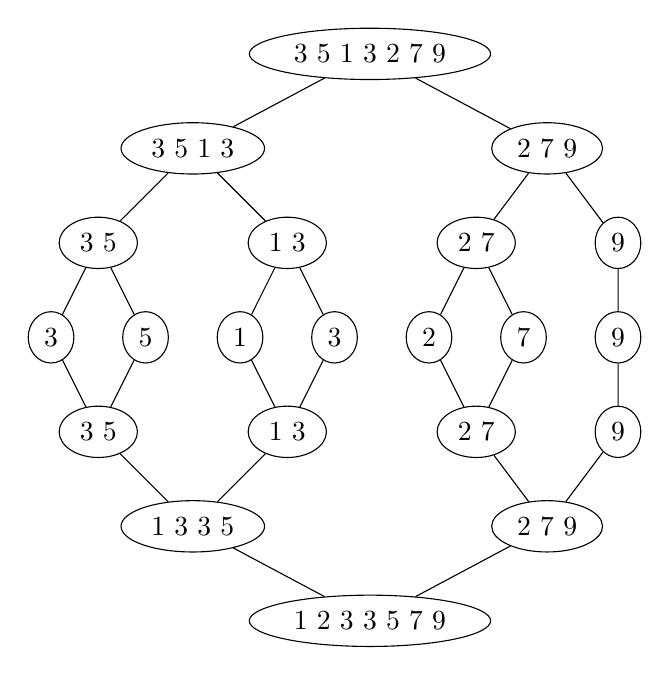
\begin{tikzpicture}[scale=1.2]
	\node [draw,ellipse] at (3.375,3) (head) {3 5 1 3 2 7 9};
	\node [draw,ellipse] at (1.5,2) (1) {3 5 1 3};
	\node [draw,ellipse] at (5.25,2) (2) {2 7 9};
	\node [draw,ellipse] at (.5,1) (3) {3 5};
	\node [draw,ellipse] at (2.5,1) (4) {1 3};
	\node [draw,ellipse] at (4.5,1) (5) {2 7};
	\node [draw,ellipse] at (6,1) (6) {9};
	\node [draw,ellipse] at (0,0) (7) {3};
	\node [draw,ellipse] at (1,0) (8) {5};
	\node [draw,ellipse] at (2,0) (9) {1};
	\node [draw,ellipse] at (3,0) (10) {3};
	\node [draw,ellipse] at (4,0) (11) {2};
	\node [draw,ellipse] at (5,0) (12) {7};
	\node [draw,ellipse] at (6,0) (13) {9};
	\node [draw,ellipse] at (.5,-1) (14) {3 5};
	\node [draw,ellipse] at (2.5,-1) (15) {1 3};
	\node [draw,ellipse] at (4.5,-1) (16) {2 7};
	\node [draw,ellipse] at (6,-1) (17) {9};
	\node [draw,ellipse] at (1.5, -2) (18) {1 3 3 5};
	\node [draw,ellipse] at (5.25, -2) (19) {2 7 9};
	\node [draw,ellipse] at (3.375,-3) (20) {1 2 3 3 5 7 9};

	\path [draw] (1) -- (head) -- (2);
	\path [draw] (3) -- (1) -- (4);
	\path [draw] (5) -- (2) -- (6);
	\path [draw] (7) -- (3) -- (8);
	\path [draw] (9) -- (4) -- (10);
	\path [draw] (11) -- (5) -- (12);
	\path [draw] (13) -- (6);
	\path [draw] (7) -- (14) -- (8);
	\path [draw] (9) -- (15) -- (10);
	\path [draw] (11) -- (16) -- (12);
	\path [draw] (13) -- (17);
	\path [draw] (14) -- (18) -- (15);
	\path [draw] (16) -- (19) -- (17);
	\path [draw] (18) -- (20) -- (19);
	\end{tikzpicture}\\*
\newline
Quicksort (using the first element in the list as a pivot):\\*
\newline
	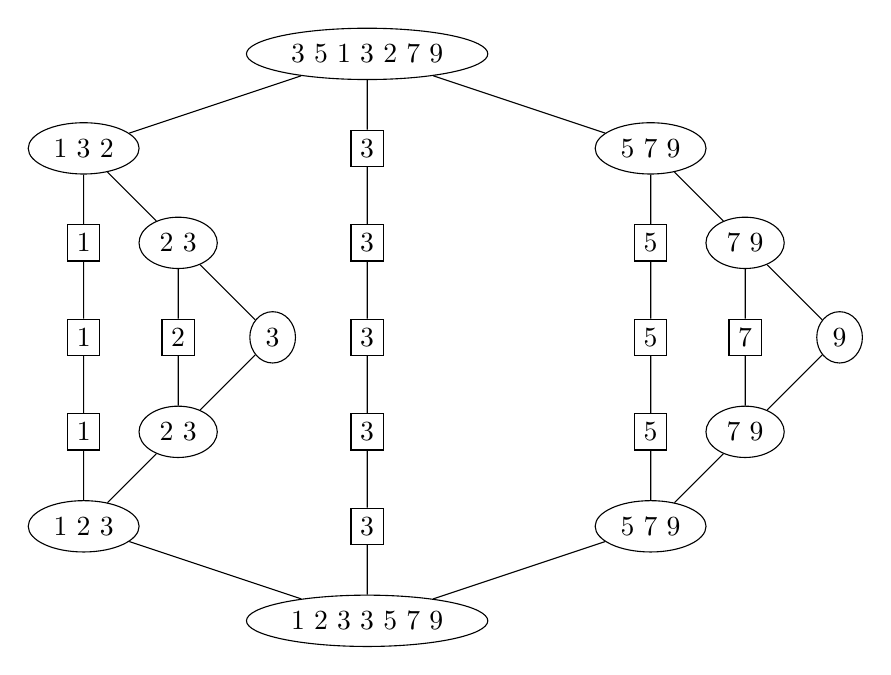
\begin{tikzpicture}[scale=1.2]
	\node [draw] at (1,0) (1) {1};
	\node [draw] at (2,0) (2) {2};
	\node [draw,ellipse] at (3,0) (3) {3};
	\node [draw] at (4,0) (4) {3};
	\node [draw] at (7,0) (5) {5};
	\node [draw] at (8,0) (6) {7};
	\node [draw,ellipse] at (9,0) (7) {9};
	\node [draw] at (1,1) (8) {1};
	\node [draw, ellipse] at (2,1) (9) {2 3};
	\node [draw] at (4,1) (10) {3};
	\node [draw] at (7,1) (11) {5};
	\node [draw,ellipse] at (8,1) (12) {7 9};
	\node [draw, ellipse] at (1,2) (13) {1 3 2};
	\node [draw] at (4,2) (14) {3};
	\node [draw,ellipse] at (7,2) (15) {5 7 9};
	\node [draw,ellipse] at (4,3) (16) {3 5 1 3 2 7 9};
	\node [draw] at (1,-1) (17) {1};
	\node [draw,ellipse] at (2,-1) (18) {2 3};
	\node [draw] at (4, -1) (19) {3};
	\node [draw] at (7,-1) (20) {5};
	\node [draw, ellipse] at (8,-1) (21) {7 9};
	\node [draw, ellipse] at (1,-2) (22) {1 2 3};
	\node [draw] at (4,-2) (23) {3};
	\node [draw, ellipse] at (7,-2) (24) {5 7 9};
	\node [draw, ellipse] at (4,-3) (25) {1 2 3 3 5 7 9};

	\path [draw] (1) -- (8) -- (13);
	\path [draw] (2) -- (9);
	\path [draw] (3) -- (9) -- (13);
	\path [draw] (4) -- (10) -- (14) -- (16);
	\path [draw] (5) -- (11) -- (15);
	\path [draw] (6) -- (12);
	\path [draw] (7) -- (12) -- (15) -- (16);
	\path [draw] (13) -- (16);

	\path [draw] (1) -- (17) -- (22);
	\path [draw] (2) -- (18);
	\path [draw] (3) -- (18) -- (22) -- (25);
	\path [draw] (4) -- (19) -- (23) -- (25);
	\path [draw] (5) -- (20) -- (24);
	\path [draw] (6) -- (21);
	\path [draw] (7) -- (21) -- (24) -- (25);

	\end{tikzpicture}
\end{answer}


\section*{Heaps and Heapsort}



\item For a binary heap containing $n$ elements, what is the maximum number of swaps occurring after an insert operation? \\
\begin{answer}
log$_{\textrm{2}}$ (n + 1), rounded down.
\end{answer}



\item Given a node in an array-based binary heap at index $i$, where are the indices of both its children? What is the index of its parent? \\
\begin{answer}
The children are at $2i+1$ and $2i+2$. The parent is at $\lfloor\frac{i-1}{2}\rfloor$.

\marginpar{\small\em Note that in a 1 indexed array system, the children would be at $2i$ and $2i+1$.  The parent would be at $\lfloor\frac{i}{2}\rfloor$.} 
\end{answer}



\item Run a heap sort on the following list: [3,5,1,3,2,7,9], showing the heap at each stage. Be sure to heapify the list first. \\
\begin{answer}
Heapify:  \newline
	[\underline{3}, 5, 1, 3, 2, 7, 9] \newline
	[\underline{3},\underline{5}, 1, 3, 2, 7, 9] \newline
	[\underline{1}, \underline{5}, \underline{3}, 3, 2, 7, 9] \newline
	[\underline{1}, \underline{3}, \underline{3}, \underline{5}, 2, 7, 9] \newline
	[\underline{1}, \underline{2}, \underline{3}, \underline{5}, \underline{3}, 7, 9] \newline
	[\underline{1}, \underline{2}, \underline{3}, \underline{5}, \underline{3}, \underline{7}, 9] \newline
	[\underline{1}, \underline{2}, \underline{3}, \underline{5}, \underline{3}, \underline{7}, \underline{9}] \newline 

Sort: \newline
	[\underline{2}, \underline{3}, \underline{3}, \underline{5}, \underline{9}, \underline{7}, 1] \newline
	[\underline{3}, \underline{3}, \underline{7}, \underline{5}, \underline{9}, 2, 1] \newline
	[\underline{3}, \underline{5}, \underline{7}, \underline{9}, 3, 2, 1] \newline
	[\underline{5}, \underline{9}, \underline{7}, 3, 3, 2, 1] \newline
	[\underline{7}, \underline{9}, 5, 3, 3, 2, 1] \newline
	[\underline{9}, 7, 5, 3, 3, 2, 1] \newline
	[9, 7, 5, 3, 3, 2, 1] \newline
\end{answer}



\end{enumerate}
\end{document}

Topics for this exam:
	- Java basics
		1, 2, 3, 4
	- Classes
	- Inheritance (interfaces & subclasses)
		5?, 6, 7, 8, 9
	- O(NlogN) sorts... mergesort and quicksort
		10, 11, 12, 13, 14, 15
	- Hashing
	- Heaps
		16, 17, 18

1) == vs .equals()
2) protected variables
3) class vs object
4) constants vs normal vars
5) overriding vs overloading methods
6) polymorphism
7) abstract class vs interface
8) "What gets printed by the following code?" ... branches of classes
9) Given code of inheritance/interfaces, find errors.
10) time complexity for different sort algorithms
11) quicksort definition
12) quicksort time complexity
13) quicksort worst-case explanation
14) quicksort (pivot selection)
15) perform mergesort and quicksort on given set of values
16) heap insertion
17) parent/child indeces in heap
18) run heapsort on given set of values